\subsection{
  Replies to comments received from Scott Oser - Feb. 08, 2014}

\begin{enumerate}

  % ........................................................................................................
  \vspace{5 mm}
\item
  {\em
    The 1D F-C VALOR contours are about 10\% smaller than those of the KDI analysis.  Does anyone know why?
  }\\
  \\

  There is a only a difference in the limits for $\sin^{2}\theta_{23}$. The limits for $|\Delta m_{32}^{2}|$ and $|\Delta m_{31}^{2}|$ are identical.
  We had noticed this difference ourselves. We are not sure of the reason for it, but we note the following differences between the KDI and VALOR results:

  \begin{itemize}
  \item  The VALOR $\Delta \chi^2$ curves in $\sin^{2}\theta_{23}$ from the data fit are slightly tighter than the KDI curves, as can be seen in
    Figs.\ \ref{fig:profile_mix23_normal} and \ref{fig:profile_mix23_inverted} of this note.
    It is possible that this difference is related to the result of a study by Minamino-san during the Run 1-3 analysis. He found that the VALOR 2D 
    constant-$\Delta \chi^{2}$ contour was slightly tighter in $\sin^{2}(2\theta_{23})$ than the KDI contour since VALOR uses a binned fit and KDI an 
    unbinned one. Please see \url{http://www.t2k.org/asg/oagroup/meeting/2013/20130509/diff\_KIT\_VaLOR\_20130511.pdf}.
    This study has been repeated with the same conclusion by Taritree for the Run 1-4 contours in $\sin^2\theta_{23}$,
    and can be seen on page 17 of \url{http://www.t2k.org/asg/oagroup/meeting/2013/2013-12-05/KDIStatus}.

    The VALOR and KDI $\Delta \chi^2$ curves in $|\Delta m_{32}^{2}|$ and $|\Delta m_{31}^{2}|$ from the data fit are more similar, as can be seen in
    Figs.\ \ref{fig:profile_dm32sq_normal} and \ref{fig:profile_dm32sq_inverted} of this note.
    
  \item A comparison of all $\Delta \chi^{2}_{crit}$ values from both KDI and VALOR are shown in Figs.\ \ref{fig:critical_mix23_normal}-\ref{fig:critical_dm32sq_inverted}
    of this note.
    They are, for the most part, consistent.
    The only difference is that the 90\% $\Delta \chi^{2}_{crit}$ values is higher for VALOR than KDI near the best-fit point in $\sin^2\theta_{23}$,
    but are consistent in the region where the 90\% limits occur.

  \item VALOR found a critical value of $\Delta \chi^2$ every 0.0100 in $\sin^{2}\theta_{23}$, whereas KDI found one every 0.0125.

  \item VALOR found a value of profile $\Delta \chi^2$ every 0.0010 in $\sin^{2}\theta_{23}$, whereas KDI found one every 0.0125.
    
  \end{itemize}

  It is possible that the difference in the 1D limits in $\sin^{2}\theta_{23}$ is due to one of these points, or it could be due to a combination of more than one of them. 

  %%%%%%%%%%% profile likelihood
  
  \begin{figure*}[htb]
    \begin{minipage}[t]{0.48\linewidth}
      \center
      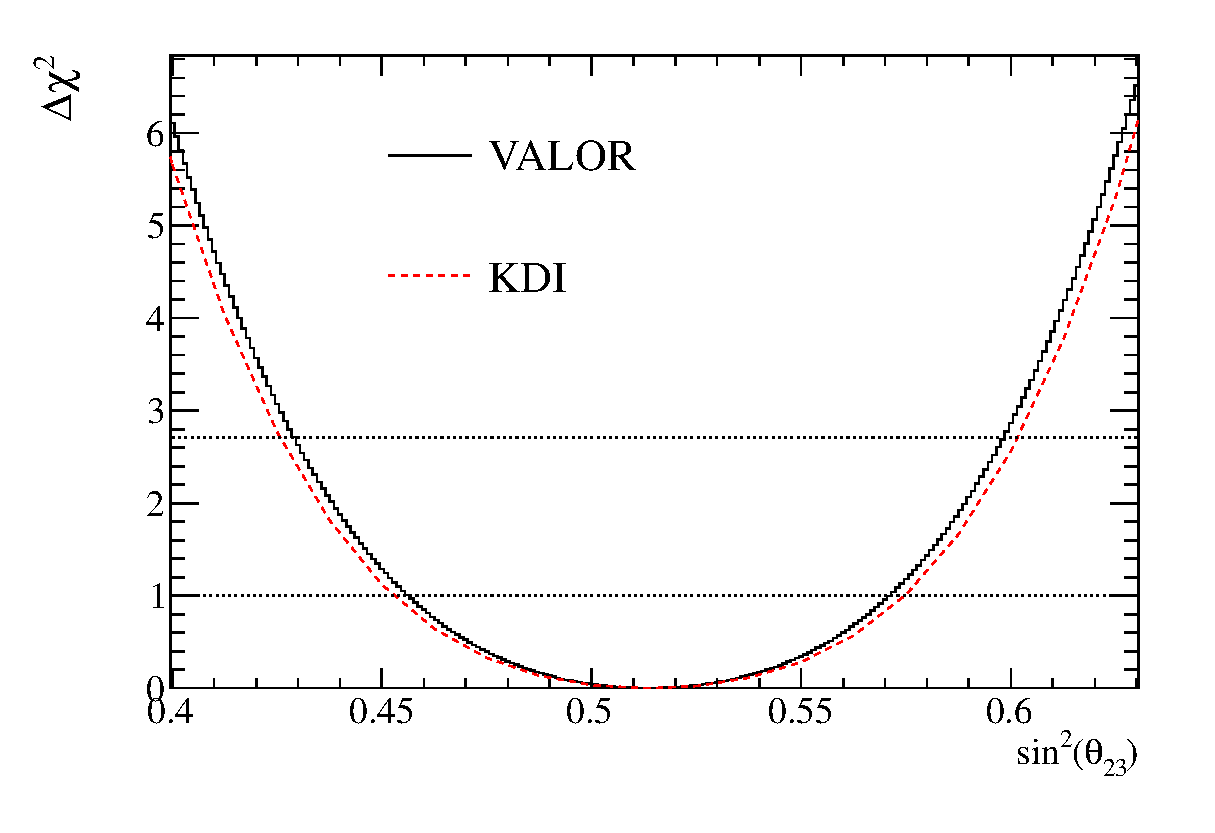
\includegraphics[width=20pc]{./images/dchisq_profiles_wkdi_mix23}
      \caption {
        Profile $\Delta \chi^2$, as a function of $\sin^2\theta_{23}$ for both VALOR and KDI fits.
        The 68\% and 90\% critical constant-$\Delta\chi^2$ values for one degree of freedom are shown as horizontal dotted lines.
        The normal mass hierarchy is assumed.
      }
      \label{fig:profile_mix23_normal}
    \end{minipage}
    \hspace{0.06\linewidth}
    \begin{minipage}[t]{0.48\linewidth}
      \center
      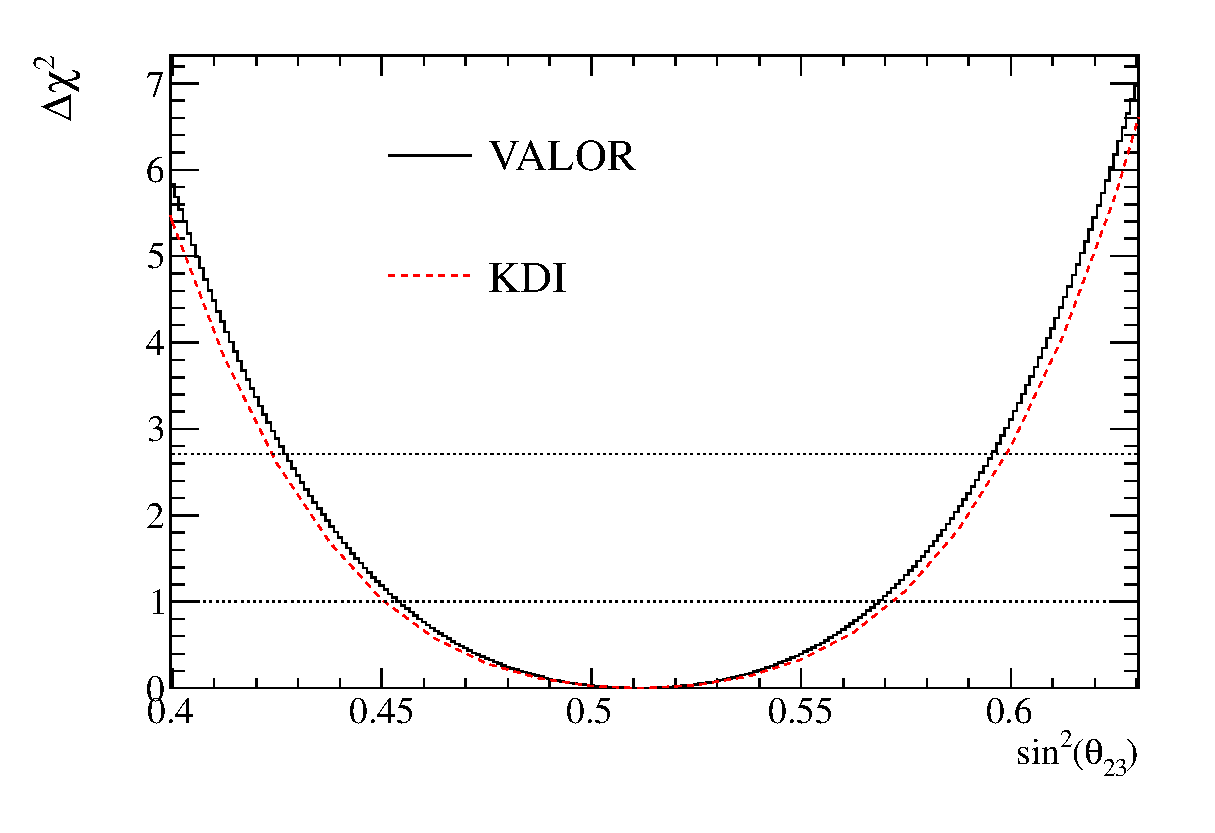
\includegraphics[width=20pc]{./images/dchisq_profiles_wkdi_mix23_inverted}
      \caption {
        Profile $\Delta \chi^2$, as a function of $\sin^2\theta_{23}$ for both VALOR and KDI fits.
        The 68\% and 90\% critical constant-$\Delta\chi^2$ values for one degree of freedom are shown as horizontal dotted lines.
        The inverted mass hierarchy is assumed.
      }
      \label{fig:profile_mix23_inverted}
    \end{minipage}
    \vfill
        \begin{minipage}[t]{0.48\linewidth}
      \center
      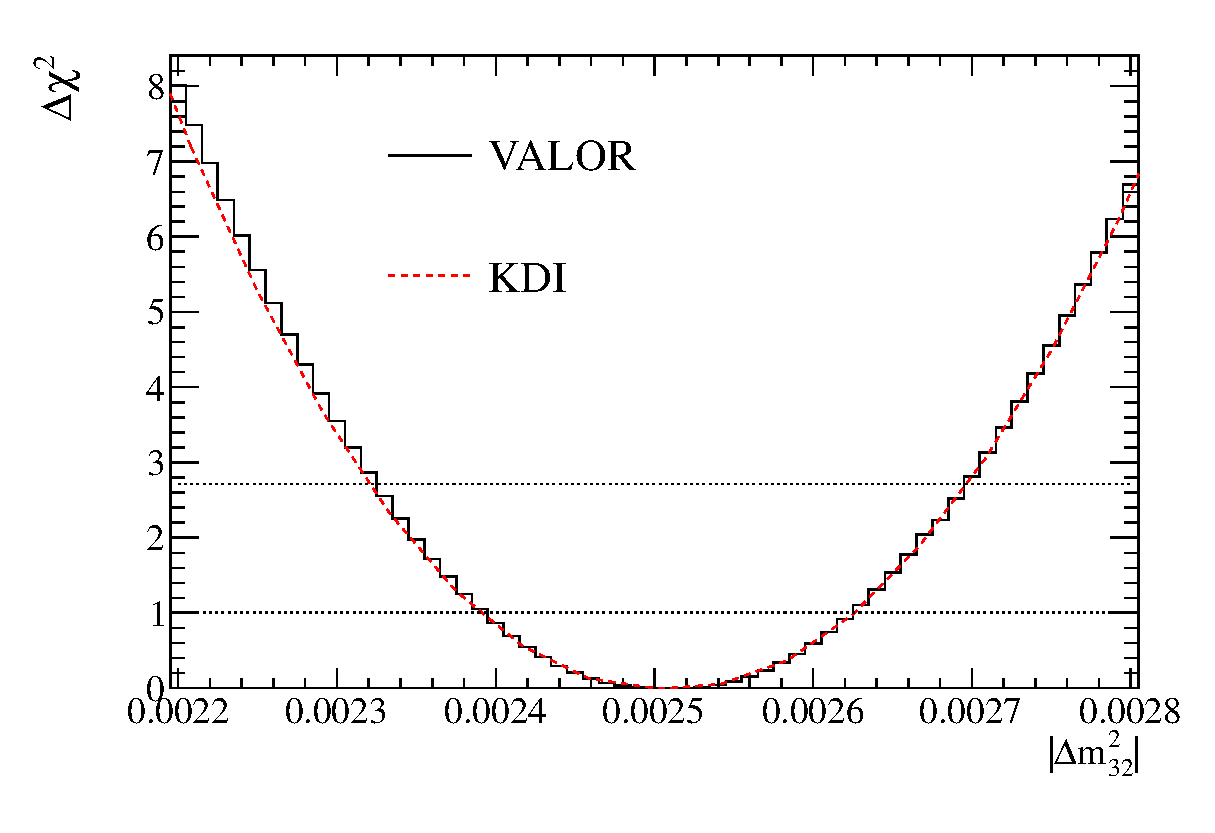
\includegraphics[width=20pc]{./images/dchisq_profiles_wkdi_dm32sq}
      \caption {
        Profile $\Delta \chi^2$, as a function of $|\Delta m_{32}^{2}|$ for both VALOR and KDI fits.
        The 68\% and 90\% critical constant-$\Delta\chi^2$ values for one degree of freedom are shown as horizontal dotted lines.
        The normal mass hierarchy is assumed.
      }
      \label{fig:profile_dm32sq_normal}
    \end{minipage}
    \hspace{0.06\linewidth}
    \begin{minipage}[t]{0.48\linewidth}
      \center
      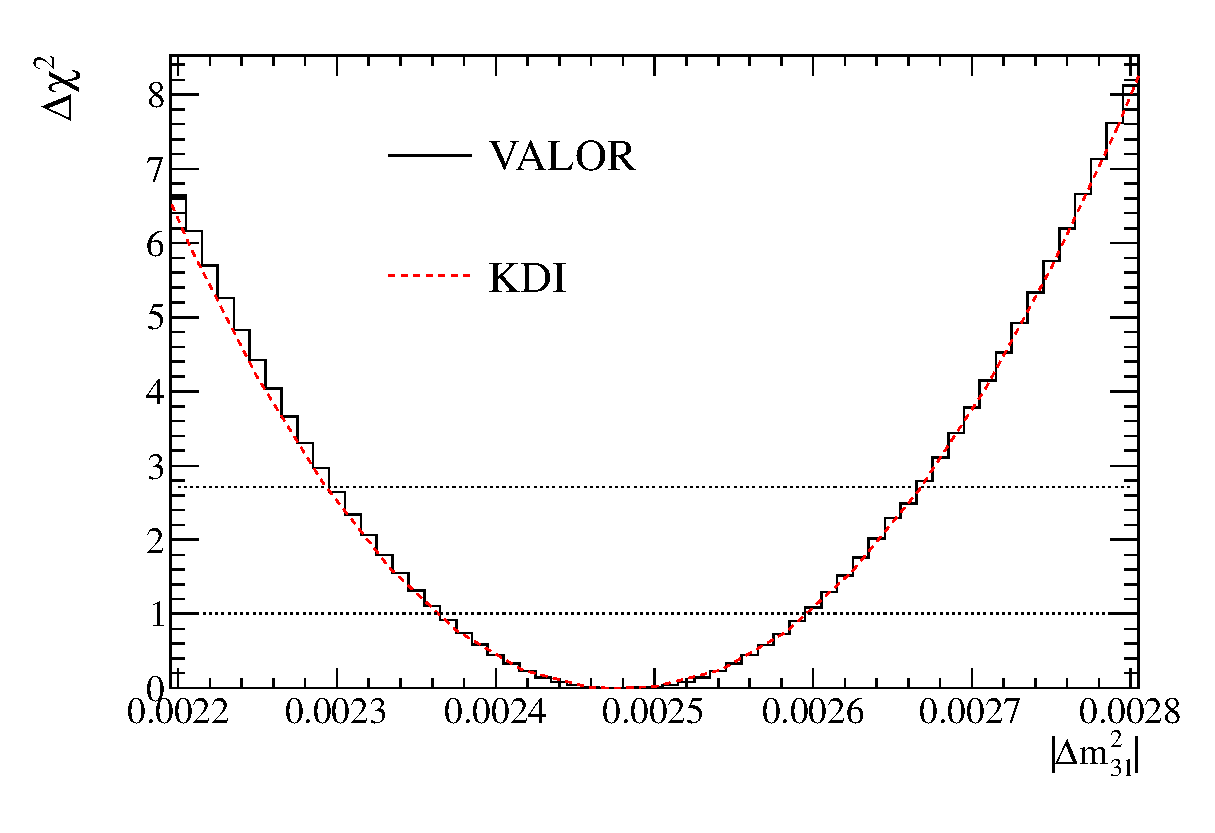
\includegraphics[width=20pc]{./images/dchisq_profiles_wkdi_dm32sq_inverted}
      \caption {
        Profile $\Delta \chi^2$, as a function of $|\Delta m_{31}^{2}|$ for both VALOR and KDI fits.
        The 68\% and 90\% critical constant-$\Delta\chi^2$ values for one degree of freedom are shown as horizontal dotted lines.
        The inverted mass hierarchy is assumed.
      }
      \label{fig:profile_dm32sq_inverted}
    \end{minipage}
  \end{figure*}

  %%%%%%%%%%%%% dchisq critical

  \begin{figure*}[htb]
    \begin{minipage}[t]{0.48\linewidth}
      \center
      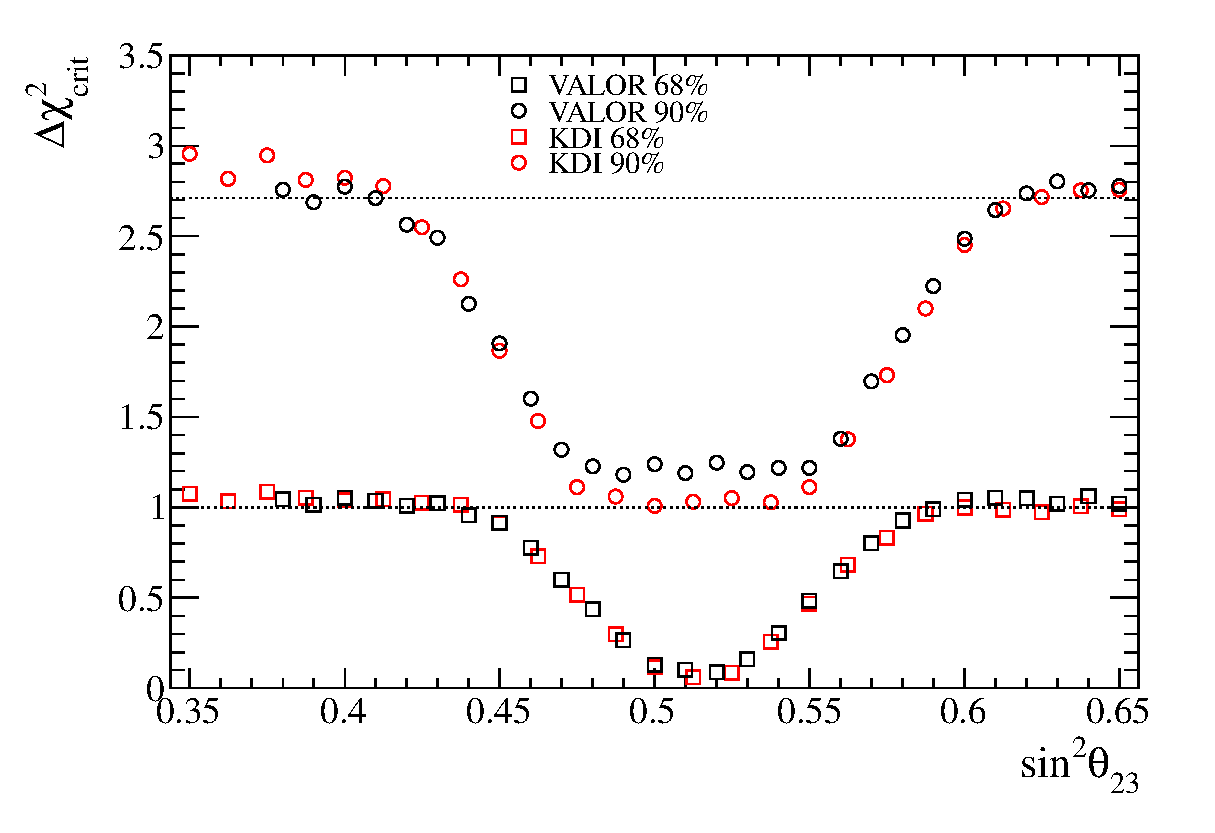
\includegraphics[width=20pc]{./images/dchisq_critical_line_wkdi_mix23_nh}
      \caption {
        $\Delta \chi^2_{crit}$, as a function of $\sin^2\theta_{23}$ for both VALOR and KDI fits.
        The 68\% and 90\% critical constant-$\Delta\chi^2$ values for one degree of freedom are shown as horizontal dotted lines.
        The normal mass hierarchy is assumed.
      }
      \label{fig:critical_mix23_normal}
    \end{minipage}
    \hspace{0.06\linewidth}
    \begin{minipage}[t]{0.48\linewidth}
      \center
      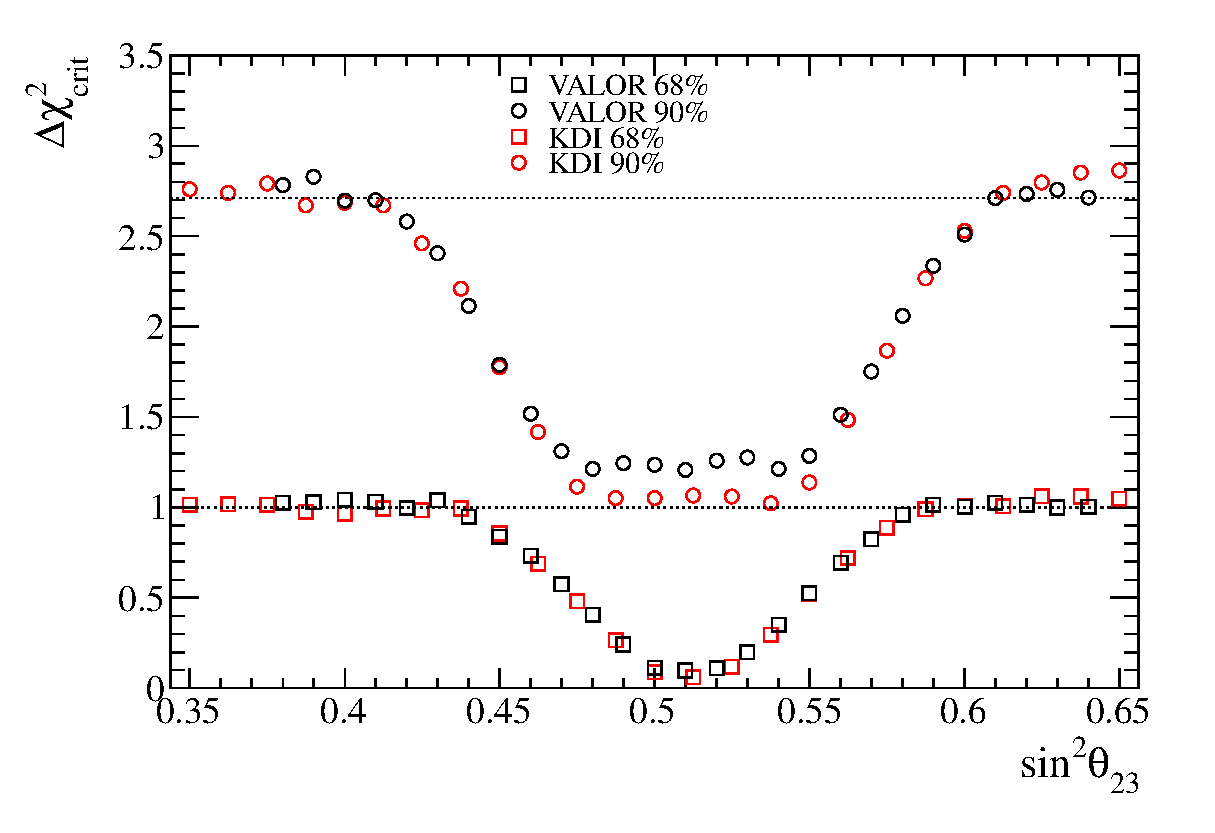
\includegraphics[width=20pc]{./images/dchisq_critical_line_wkdi_mix23_ih}
      \caption {
        $\Delta \chi^2_{crit}$, as a function of $\sin^2\theta_{23}$ for both VALOR and KDI fits.
        The 68\% and 90\% critical constant-$\Delta\chi^2$ values for one degree of freedom are shown as horizontal dotted lines.
        The inverted mass hierarchy is assumed.
      }
      \label{fig:critical_mix23_inverted}
    \end{minipage}
    \vfill
        \begin{minipage}[t]{0.48\linewidth}
      \center
      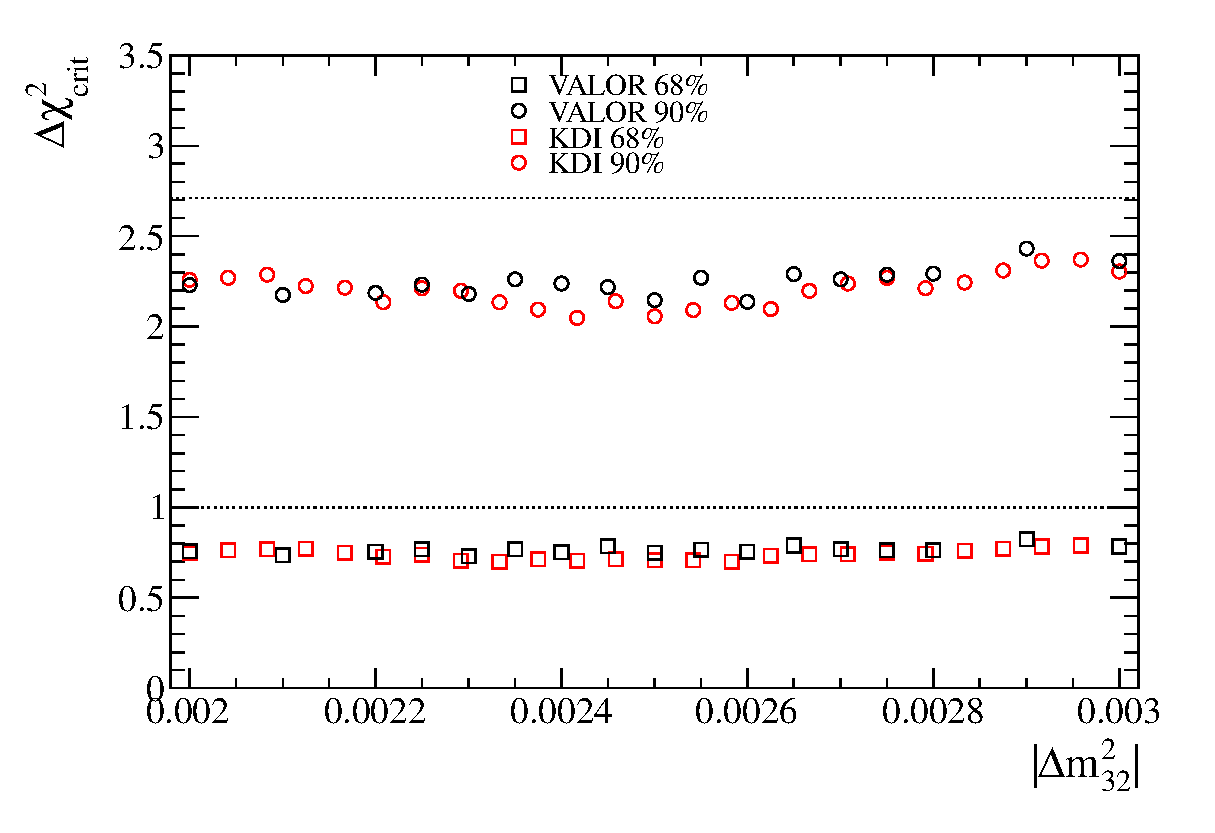
\includegraphics[width=20pc]{./images/dchisq_critical_line_wkdi_dm32sq_nh}
      \caption {
        $\Delta \chi^2_{crit}$, as a function of $|\Delta m_{32}^{2}|$ for both VALOR and KDI fits.
        The 68\% and 90\% critical constant-$\Delta\chi^2$ values for one degree of freedom are shown as horizontal dotted lines.
        The normal mass hierarchy is assumed.
      }
      \label{fig:critical_dm32sq_normal}
    \end{minipage}
    \hspace{0.06\linewidth}
    \begin{minipage}[t]{0.48\linewidth}
      \center
      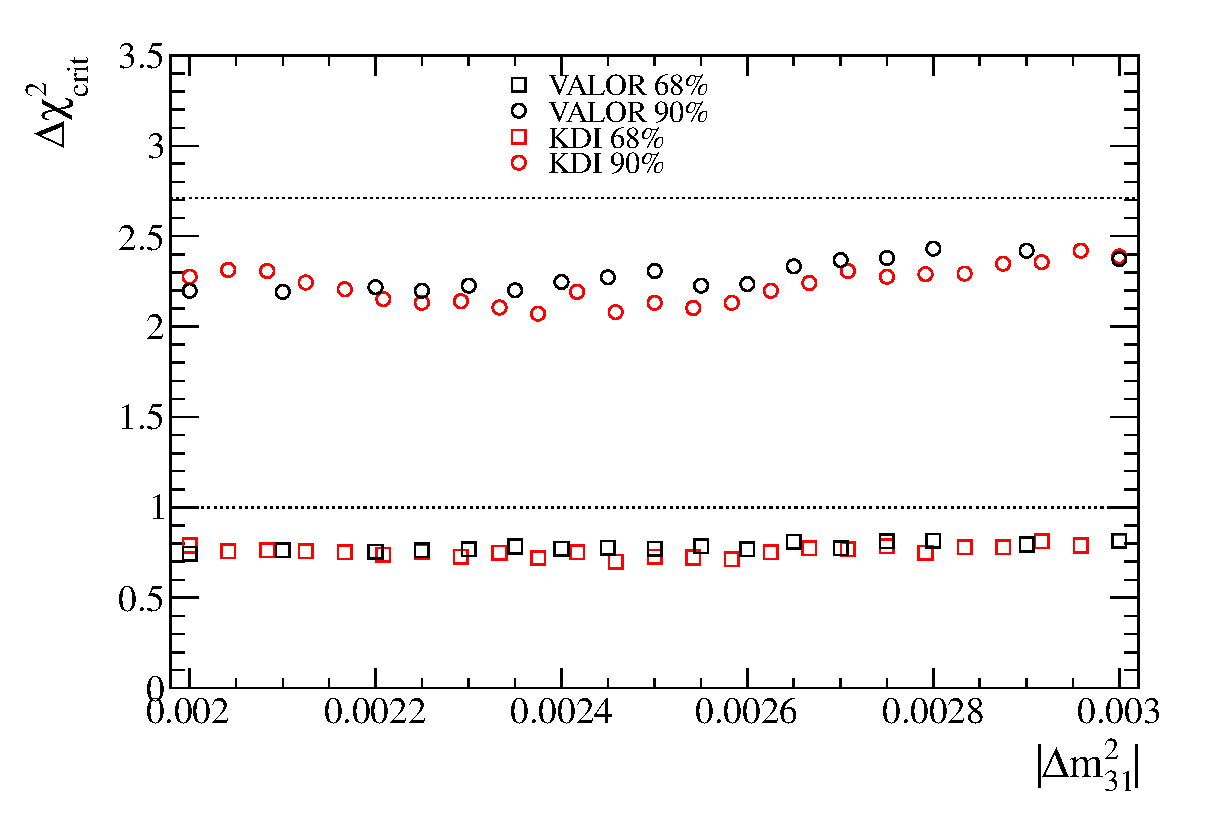
\includegraphics[width=20pc]{./images/dchisq_critical_line_wkdi_dm32sq_ih}
      \caption {
        $\Delta \chi^2_{crit}$, as a function of $|\Delta m_{31}^{2}|$ for both VALOR and KDI fits.
        The 68\% and 90\% critical constant-$\Delta\chi^2$ values for one degree of freedom are shown as horizontal dotted lines.
        The inverted mass hierarchy is assumed.
      }
      \label{fig:critical_dm32sq_inverted}
    \end{minipage}
  \end{figure*}

  
  % ........................................................................................................
  \vspace{5 mm}
\item
  {\em
    p. 20, Table 4,\\
    regarding the $M_A^{RES}$ value: TN-166 says the prior value for this parameter was 1.41, and fit value was 0.965, so the ratio should be 0.68, not 0.797 as listed in this table.  Please explain this discrepancy.
  }\\
  \\
  The number listed in Tab.\ 4 is $x_{MARES}$, defined such that $M_A^{RES}(\textrm{MC tuned}) = x_{MARES} M_A^{RES}(\textrm{MC nominal})$.
  $M_A^{RES}(\textrm{MC nominal})$ is the value of $M_A^{RES}$ that the SK MC was generated with, and this value is 1.21 GeV/c$^4$.
  Therefore the ratio $x_{MARES} = 0.965/1.21 = 0.797$ is consistent and correct.
  
  % ........................................................................................................
  \vspace{5 mm}
\item
  {\em
    line 574:\\
    Please state which specific input points were tested.
  }\\
  \\
  These have been added to v3 of the note.

  % ........................................................................................................
  \vspace{5 mm}
\item
  {\em
    lines 628-630:\\
    how could it ever happen that the predicted number of events would be negative?
  }\\
  \\
  When there a large enough negative tweak in systematic parameters (excluding SK energy scale \& oscillation parameters), the event weight returned can be negative.
  For example, the CC coherent cross section normalisation has a value of 100\%, so a tweak of -2$\sigma$ leads to a weight of -1.00 for CC coherent modes,
  but (assuming all other systematics nominal) the total number of $E_{reco}$ events is positive.
  Therefore a very large tweak and/or a combination of negative weights is required.
  
  This was a bigger effect in the 2012 analysis, where the SK NC efficiency parameter was approximately twice as big (111\%), and made the first bin negative at $>-$2$\sigma$.
  In this analysis, it is a smaller effect; out of a test of 100000 random tweaks of all systematics performed at
  $\sin^2\theta_{23} = 0.5$ and $|\Delta m^2_{32}| = 2.40 \times 10^{-3}$ eV$^2$/c$^4$, only 175 (0.18\%) result in negative events.

  % ........................................................................................................
  \vspace{5 mm}
\item
  {\em
    p. 49, Table 12,\\
    last line: the value of $\sin^2(\theta_{23})=1$ is probably a typo, I hope.
  }\\
  \\
  Yes, the value $\sin^2(2\theta_{23})=1$ was written in the table; it should of been $\sin^2\theta_{23}=0.514$. Fixed.
  
  % ........................................................................................................
  \vspace{5 mm}
\item
  {\em
    p. 71, Fig 54:\\
    I think the y axis is $\Delta m^2_{13}$, actually
  }\\
  \\
  Correct. This has been fixed. The $\Delta m^2$ axes of Figs.\ 50, 58, 61, 62, 67, 81 have also been updated.
    
  % ........................................................................................................
  \vspace{5 mm}
\item
  {\em
    Fig 81: I'm not quite sure if I should make this comment, at the risk of derailing people on a statistics question.  But this plot does give me pause and suggests to me that we really ought to question whether Feldman-Cousins is worth all the trouble.  Feldman \& Cousins themselves say that when the limit is noticeably better than the sensitivity then the limit should be taken with a grain of salt.  Basically, F-C has trouble giving sensible limits for the case that the data fluctuates below the prediction.  This is unfortunately exactly the case we have for our T2K data.  While it is true that F-C will give correct coverage for an ensemble of data sets, in practice, for the actual data that T2K actually has accumulated, this figure suggests that the limits are probably too small and should not be taken too seriously.  I seriously think we should consider not using F-C in future papers for this reason.  You are welcome to comment on this or ignore as you prefer.
  }\\
  \\
  We use the Feldman \& Cousins method because that was the recommendation of the $\nu_\mu$ contour committee (\url{http://www.t2k.org/asg/TFs/contour/ASG-Conveners-Report}).
  It may be opening a can of worms (it is a tricky issue of deciding how to do an analysis once we have seen the data),
  but the discussion could be reopened within the oscillation analysis group for the Run 1-5 analyses.
  % The p-value isn't really that bad, $\gtsim 20\%$, and so while the data is near the limit of the model, it doesn't seem to go much beyond it.

    
\end{enumerate}
  
